\documentclass[tikz,border=8pt]{standalone}
\usepackage{amsmath}
\begin{document}
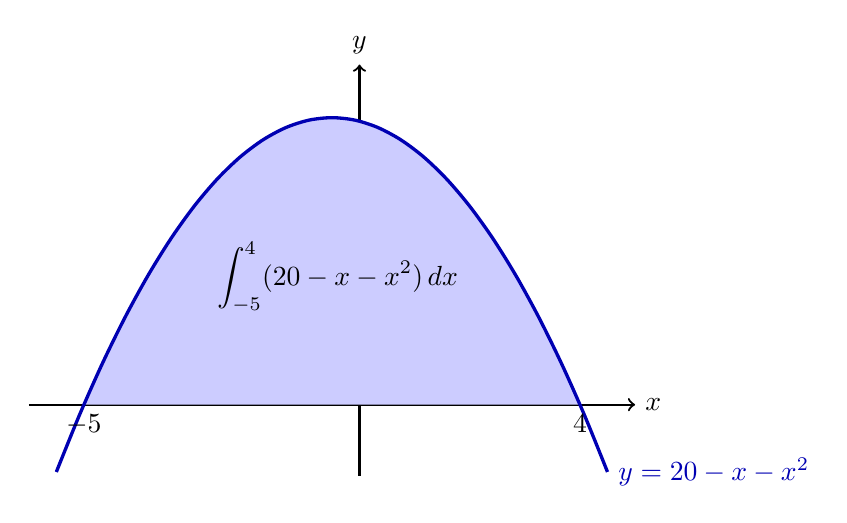
\begin{tikzpicture}[xscale=0.7,yscale=0.18]
\draw[->,thick] (-6,0)--(5,0) node[right] {$x$};
\draw[->,thick] (0,-5)--(0,24) node[above] {$y$};
\fill[blue!20] (-5,0)--plot[smooth,domain=-5:4] (\x,{20-\x-\x*\x})--(4,0)--cycle;
\draw[very thick,blue!70!black] plot[smooth,domain=-5.5:4.5] (\x,{20-\x-\x*\x}) node[right] {$y=20-x-x^2$};
\node[below] at (-5,0) {$-5$}; \node[below] at (4,0) {$4$};
\node at (-0.4,9) {$\displaystyle \int_{-5}^4(20-x-x^2)\,dx$};
\end{tikzpicture}
\end{document}